%\thispagestyle{empty}
\chapter{Методы изучения волновых движений в жидкости конечной глубины} \label{chapt1}

\section{Введение}

В данной главе будут показаны средства и методы изучения волнения:
\begin{enumerate}
  \item Уравнения Эйлера в трехмерном и двумерном виде.
  \item Линеаризация уравнения Эйлера и обезразмеривание.
  \item Связь колебаний уровня моря с вариациями придонного давления
  \item Методы хранения База данных
  \item Методы Пересчета из придонного давления в обычное
  \item Методы учета влияния нелинейности
\end{enumerate}
%\section{Теоретические модели волновых движений в жидкости конечной глубины}
\section{Уравнения идеальной жидкости. Полнонелинейная модель}

%%%%Переработать текст изменить чтоб без плагиата, и с другими переменными

Опишем математическую модель движения жидкости, используя ряд упрощающих предположений во-первых будем считать жидкость сплошной и однородной средой. При этом будем описывать состояние жидкости, занимающей объем $V$, с помощью поля скоростей:
$$
\overrightarrow v(x,y,z)=(u,v,w), (x,y,z)\in V,
$$

Мы рассматриваем нестационарное течение жидкости, а значит поле скоростей будет зависеть от
вре\-ме\-ни: $(u(x,y,z,t),v(x,y,z,t),w(x,y,z,t))$. Область, занимаемая жидкостью, также может зависеть от времени (в частности, в задачах со свободной поверхностью): $V=V(t)$.

\begin{figure} [h]
  \center
  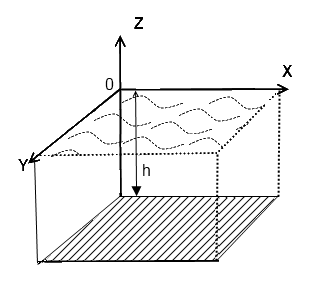
\includegraphics [width=0.7\linewidth] {model.png}
  \caption{Система координат в жидкости конечной глубины}
  \label{img:anivaMap}
\end{figure}
\FloatBarrier

Во-вторых будет рассматриваться жидкость при отсутствии вязкости. Известно, что  вода имеет очень небольшой коэффициент вязкости:
$\nu=1,005~\cdot~10^{-3}\ \mbox{Па}\cdot\mbox{с}$\footnote{В Международной системе (СИ) единицей вязкости является паскаль-секунда:
$1\mbox{Па}\cdot\mbox{с}=1\mbox{кг}/(\mbox{м}\cdot\mbox{с})$}, для сравнения глицерин имеет коэффициент вязкости $\nu=4,22\ \mbox{Па}\cdot\mbox{с},$ см. \cite{loyts}. Принятие коэффициента вязкости равным нулю приводит к существенному упрощению уравнений и граничных условий.

Так как в текущей работе изучаются поверхностные волны, то будем рассматривать тяжелую жидкость, находящуюся с однородном поле силы тяжести. Рассматриваемая жидкость будет обладать однородной плотностью $\rho$.

В-третьих будем считать жидкость несжимаемой. Тогда закон сохранения массы для любого объёма движущейся жидкости в переменных Эйлера выражается формулой
\begin{equation}\label{eq:divNull}
div\overrightarrow v(x,y,z,t)=u_x+v_y+w_z=0,\quad
x,y,z\in V(t).
\end{equation}

Далее рассмотрим основные уравнения движения, которые в совокупности с условием неразрывности \eqref{eq:divNull} описывают динамику идеальной несжимаемой жидкости. Данная система уравнений носит название системы уравнений Эйлера:
\begin{equation}\label{eq:euler}
\begin{cases}
u_t + uu_x + vu_y + wu_z + P_x/\rho = 0, & \\
v_t + uv_x + vv_y + wv_z + P_y/\rho = 0, & \\
w_t + uw_x + vw_y + ww_z + P_z/\rho = -g, & \\
u_x+v_y+w_z=0, & (x,y,z,t)\in V(t)  \\
\end{cases}
\end{equation}
где $g$ - ускорение свободного падения, скалярная функ\-ция~$P(x,y,z,t)$ - давление, $\rho$ - плотность.
Система координат связана с невозмущенной океанической
поверхностью, ось $z$ направлена вертикально вверх.

Система уравнений Эйлера~\eqref{eq:euler} должна быть дополнена граничными условиями на дне и на свободной поверхности. На дне это условие непротекания жидкости, которое означает что вертикальная скорость на дне равна нулю:
\begin{equation}\label{eq:granUslBottom}
  w{|_{z=-h}}=0,
\end{equation}
на свободной поверхности $z=\eta(x,y,z)$ это кинематическое условие:
\begin{equation}\label{eq:kinematGranUsl}
  {\frac{d\eta}{dt}}{|_{z=\eta}}={(\frac{\partial\eta}{\partial t}+u\frac{\partial\eta}{\partial x}+v\frac{\partial\eta}{\partial y})}|_{z=\eta}=w,
\end{equation}
а также динамическое условие:
\begin{equation}\label{eq:dynGranUsl}
  {P}|_{z=\eta}=P_{atm},
\end{equation}

При решении задач гидродинамики, рассматриваемых в океанологии, занимаемые жидкостью областью часто имеют огромные размеры, поэтому допустимо использовать периодические граничные условия.

Несмотря на то, что в систему~\eqref{eq:euler} не входит
производная по времени от давления, уравнения Эйлера являются
эволюционной системой с выделенной переменной времени $t$.

%
%При изучении динамики эволюционных систем необходимо
%задавать начальные условия
%\begin{equation}\label{eq_ev}
%\begin{array}{cc}
%\overrightarrow v(x,y,z, 0)=\overrightarrow v_0(x,y,z), &  \\
% & (x,y,z\in V) \\
%P(x,y,z,0)=P_0(x,y,z).  & \\
%\end{array}
%\end{equation}
%Поскольку давление $P(x,y,z,t_0)$ может быть определено по полю
%скоростей $\overrightarrow v(x,y,z, t_0)$ при фиксированном $t_0,$ то
%начальные условия~\eqref{eq_ev} должны удовлетворять
%соответствующим условиям согласования.

Представленная система уравнений Эйлера~\eqref{eq:euler} совместно с граничными условиями~\eqref{eq:granUslBottom}-\eqref{eq:dynGranUsl} позволяет достаточно полно описывать волны на воде \cite{Sretensky}. Но также представляет собой очень сложную
математическую задачу, как в плане доказательства теорем о
существовании и единственности решений этой системы, так и с
вычислительной точки зрения. В двумерном случае результаты о
разрешимости уравнений Эйлера получены в работах \cite{Udo,Kato}.
В трехмерном случае до настоящего момента результатов о глобальной
(по времени) разрешимости уравнения Эйлера неизвестно.
Существование решений на достаточно малом временном интервале в
трехмерном случае рассматривалось в работах \cite{Gunter,Lich}.

%\subsection{Уравнения Эйлера в двумерных координатах}\label{linTheory}
%
%Предположим что волновое поле двумерное, т.е. параллельные гребни волны движутся одинаково. Таким образом используя декартовы координаты $(x,y)$ мы рассматриваем поперечное сечение волновой формы перпендикулярно линии гребня с осью $Y$ направленной вертикально вверх, и осью $X$ ориентированной в направлении движения волны.
%
%Пусть $(u(t, x, y), v(t, x, y))$ поле скоростей водного потока, предположим что морское дно является плоским и расположено на уровне $y=0$, тогда $y = h_0 + \eta(t, x)$ будет свободной поверхностью, где $h_0>0$ - средняя глубина бассейна, рассчитанная от плоского дна.  Обозначим через $P$ давление жидкости, а через $g$ - константу ускорения свободного падения. Тогда основные уравнения описывающие волны в жидкости можно представить так \cite{Esher_Schlurmann_2008} \cite{17_Johnson}:
%\begin{enumerate}
%  \item Уравнение Эйлера:
%  \begin{equation}\label{eq:eulerLin}
%    \begin{cases}
%        u_t + uu_x + vu_y = -P_x,  & \\
%        v_t + uv_x + vv_y = -P_y - g, & \\
%    \end{cases}
%  \end{equation}
%  \item Уравнение сохранения массы:
%  \begin{equation}\label{eq:massConserv}
%    u_x + v_y = 0
%  \end{equation}
%  \item Динамические граничные условия:
%  \begin{equation}\label{eq:dinGranCond}
%      P = P_a; y = h_0 + \eta (t, x),
%  \end{equation}
%  где $P_a$ постоянное атмосферное давление по поверхности жидкости
%  \item Кинематическое граничное условие на свободной поверхности:
%  \begin{equation}\label{eq:kinGranCond}
%       v = \eta_t + u\eta_x;  y = h_0 + \eta(t, x)
%  \end{equation}
%  \item Кинематическое граничное условие на дне:
%  \begin{equation}\label{eq:kinGranCond_Bed}
%       v = 0.
%  \end{equation}
%\end{enumerate}
%
%В текущем рассмотрении волн мы предполагаем, что в начальный момент времени $t = 0$ возмущается плоская поверхность неподвижной жидкости и далее анализируется результат этого возмущения во времени. Мы также предполагаем, что поток является безвихревым, т.е. движение потенциальное:
%$$
%u_y=v_x,
%$$

\subsection{Линейная теория} \label{sect_linTheory_norming}

Сначала мы рассмотрим линейные волны, когда в уравнениях и граничных условиях пренебрегают нелинейными членами и условия на свободной поверхности $(z=\eta)$ сносят на невозмущенную поверхность  $(z = 0)$. При этом в давлении необходимо выделить гидростатический член в явном виде:
\begin{equation}\label{eq:linPel}
  P = P_{atm}-\rho gz+P'(x,y,z,t).
\end{equation}
Кроме того, будем считать, что в океане отсутствуют какие-либо течения. Тогда в линейном приближении исходная система
уравнений имеет следующий вид:
\begin{equation}\label{eq:linEuler}
\begin{cases}
    u_t+P'_x/\rho=0, &\\
    v_t+P'_y/\rho=0, &\\
    w_t+P'_z/\rho=0, &\\
    u_x+v_y+w_z=0; &\\
\end{cases}
\end{equation}
и соответственно граничные условия:
\begin{equation}\label{eq:granUslLin}
\begin{cases}
    w|_{z=-h}=0, &\\
    \frac{\partial \eta}{\partial t}|_{z=0}=w, &\\
    P'|_{z=0}=\rho g\eta. &\\
\end{cases}
\end{equation}
Из уравнений движения в системе \eqref{eq:linEuler} вытекает также, что ротор скорости равен нулю, т.е. волновое движение в отсутствие внешних течений всегда является потенциальным. Тогда если введем потенциал скорости с помощью выражений:
\begin{equation}\label{eq:potenLin}
u=\frac{\partial \varphi}{\partial x},v=\frac{\partial \varphi}{\partial y},w=\frac{\partial \varphi}{\partial z};
\end{equation}
то можем из уравнения неразрывности в системе уравнений \eqref{eq:linEuler} получаем, что введенный потенциал поля скоростей $\varphi$ удовлетворяет уравнению Лапласа:
\begin{equation}\label{eq:laplasLin}
\frac{\partial^2 \varphi}{\partial x^2}+\frac{\partial^2 \varphi}{\partial y^2}+\frac{\partial^2 \varphi}{\partial z^2}=0.
\end{equation}
Граничные условия, представленные системой \eqref{eq:granUslLin} при этом, а также с учетом уравнения Бернулли, принимают вид:
\begin{equation}\label{eq:granUslLin1}
\begin{cases}
    \frac{\partial \varphi}{\partial z}|_{z=-h}=0, &\\
    \frac{\partial \eta}{\partial t}|_{z=0}=\frac{\partial \varphi}{\partial z},&\\
    (\frac{\partial \varphi}{\partial t}+ g\eta)|_{z=0}=0.&\\
\end{cases}
\end{equation}

Также граничные условия на свободной границе $(z=0)$ можно переписать в следующем виде:
\begin{equation}\label{eq:granUslLin2}
    (\frac{\partial^2 \varphi}{\partial t^2}+ g\frac{\partial \varphi}{\partial z})|_{z=0}=0.
\end{equation}

Таким образом можно составить замкнутую систему уравнений для определения потенциала скоростей $\varphi$:
\begin{equation}\label{eq:granUslLin1}
\begin{cases}
    \frac{\partial^2 \varphi}{\partial x^2}+\frac{\partial^2 \varphi}{\partial y^2}+\frac{\partial^2 \varphi}{\partial z^2}=0, &\\
    \frac{\partial \varphi}{\partial z}|_{z=-h}=0, &\\
    (\frac{\partial^2 \varphi}{\partial t^2}+ g\frac{\partial \varphi}{\partial z})|_{z=0}=0. &\\
\end{cases}
\end{equation}

\subsection{Монохроматическая волна}
Рассмотрим решения уравнений \eqref{eq:linEuler} и \eqref{eq:granUslLin} соответствующие линейным свободным \emph{бегущим или прогрессивным} волнам, распространяющимся вдоль оси $x$. Предположим что волновое поле двумерное, т.е. параллельные гребни волны движутся одинаково. Таким образом используя декартовы координаты $(x,z)$ мы рассматриваем поперечное сечение волновой формы перпендикулярно линии гребня с осью $Z$ направленной вертикально вверх, и осью $X$ ориентированной в направлении движения волны.

\begin{figure} [ht]
  \center
  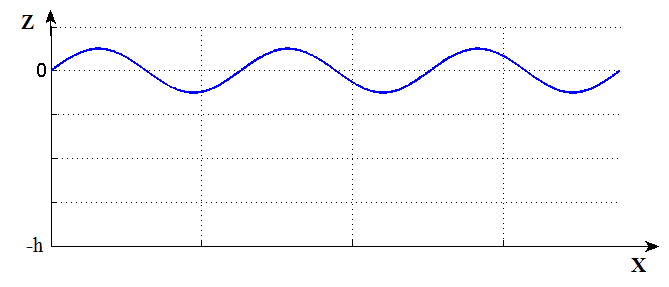
\includegraphics [width=0.8\linewidth] {systCoord.png}
  \caption{Монохроматическая волна в двумерной системе координат}
  \label{img:systCoord}
\end{figure}
\FloatBarrier

Тогда точное решение уравнений \eqref{eq:linEuler}-\eqref{eq:granUslLin} будет иметь вид:
\begin{equation}\label{eq:solveEuler}
  \begin{cases}
  u=Re(U(z))\exp[i(\omega t-kx)], & \\
  w=Re(W(z))\exp[i(\omega t-kx)], & \\
  p=Re(\rho P(z))\exp[i(\omega t-kx)], & \\
  \eta = a_0\exp(i\alpha)\exp[i(\omega t-kx)]. & \\
  \end{cases}
\end{equation}
Здесь $\omega$ -- частота; $k$ -- волновое число; $a_0$ -- амплитуда волны; $\alpha$ -- её фаза; $U(z),W(z), P(z)$ -- комплексные функции, описывающие вертикальное распределение волновых полей, их зависимость от глубины; $Re$ -- знак вещественной части получаемых выражений. Такая форма решения имеет место во всех случаях, когда исходные уравнения дополняются граничными условиями; такие задачи называются краевыми. Подставляя решение \eqref{eq:solveEuler} в систему уравнений \eqref{eq:linEuler}-\eqref{eq:granUslLin}, можно найти связь между различными характеристиками:
\begin{equation}\label{eq:connCharac}
  U(z)=\frac{1}{ik}\frac{dW}{dz}; P(z)=\frac{\omega}{ik^2}\frac{dW}{dz},
\end{equation}
а для $W$ получается краевая задача:
\begin{equation}\label{eq:WborderTask}
  \frac{d^2W}{dz^2}-k^2W=0; \\
  (W-\frac{\omega^2}{gk}\frac{dW}{dz})|_{z=0}=0,W|_{z=-h}=0.
\end{equation}

Решение этой задачи находится в явном виде:
\begin{equation}\label{eq:solveBorderTask}
W(z)=A\exp(kz)+\exp(-kz),
\end{equation}
\noindent
где константы $A$ и $B$ должны находиться из граничных условий. Подстановка \eqref{eq:solveBorderTask} в граничные условия в \eqref{eq:WborderTask} приводит к линейной однородной системе:
\begin{equation}\label{eq:findAandB}
  \begin{cases}
  A\exp(-kh)+B\exp(kh)=0,& \\
  [1-\omega^2/(gk)]A+[1+\omega^2/(gk)]B=0. & \\
  \end{cases}
\end{equation}
Решение \eqref{eq:findAandB} существует только если детерминант системы равен нулю, что приводит к следующему выражению:
\begin{equation}\label{eq:dispSootn}
  \omega^2=gk \operatorname{th} (kh).
\end{equation}
Таким образом, частота волны и ее волновое число связаны между собой дисперсионными соотношением \eqref{eq:dispSootn}.

Учитывая это константы $A$ и $B$ также связаны между собой. Используя соотношение \eqref{eq:granUslLin} можем окончательно записать полное описание свободных монохроматических волн:
\begin{equation}\label{eq:solveBorderTask1}
  \begin{cases}
  W(z)=i\omega a_0\frac{\operatorname{sh}[k(z+h)]}{\operatorname{sh}(kh)}\exp(i\alpha); & \\
  U(z)=\omega a_0\frac{\operatorname{ch}[k(z+h)]}{\operatorname{sh}(kh)}\exp(i\alpha); & \\
  P(z)=g a_0\frac{\operatorname{ch}[k(z+h)]}{\operatorname{ch}(kh)}\exp(i\alpha); & \\
  \end{cases}
\end{equation}
Либо в действительной форме:
\begin{equation}\label{eq:solveBorderTask1}
  \begin{cases}
  \eta=a_0\cos(\omega t-kx+\alpha); & \\
  w = -\omega a_0\frac{\operatorname{sh}[k(z+h)]}{\operatorname{sh}[kh]}\sin(\omega t - kx+\alpha); & \\
  u = \omega a_0\frac{\operatorname{ch}[k(z+h)]}{\operatorname{sh}[kh]}\cos(\omega t - kx+\alpha); & \\
  p = p_{atm}-\rho gz+\rho ga_0\frac{\operatorname{ch}[k(z+h)]}{\operatorname{ch}[kh]}\cos(\omega t - kx+\alpha). & \\
  \end{cases}
\end{equation}
%%Возможно надо переделать
Волнограмма в фиксированной произвольной точке представляет собой синусоиду с периодом $T=2\pi/\omega$. Максимальный размах колебаний называется высотой волны, и она, в данном случае, равна $2a_0$. Аналогичный вид имеет профиль свободной поверхности в фиксированный момент времени $t$. Расстояние между вершинами в пространстве называется длиной волны: $\lambda=2\pi/k$. Длина волны и период не могут изменяться произвольным образом, они связаны между собой дисперсионным соотношением \eqref{eq:dispSootn}. Любая точка профиля волны перемещается в пространстве со скоростью $c_{\text{фаз}}$, называется фазовой скоростью волны, она определяется как:
\begin{equation}\label{eq:fazSpeed}
  c_{\text{фаз}}=\omega/k=\sqrt{(g/k)\operatorname{th}(kh)},
\end{equation}

Поле скоростей частиц жидкости в толще воды и на ее поверхности определяется выражениями описанными в системе \eqref{eq:solveBorderTask1}. На каждом фиксированном горизонте скорости частиц описываются выражениями типа монохроматической бегущей волны, причем горизонтальная скорости синфазна со смещением поверхности, следовательно максимальное значение модуля скорости на всех горизонтах достигается при прохождении гребня и ложбины. Вертикальная скорость сдвинута по фазе на $\pi/2$ от горизонтальной скорости, так что ее максимум приходится на участки с нулевым смещением поверхности. С глубиной скорости частиц (а следовательно и смещения частиц) убывают, причем характер убывания определяется параметром $kh$ или $h/\lambda$; с уменьшением длины волны волновые возмущения все менее проникают в глубь жидкости.

Волновые возмущения давления(поправка к гидростатическому давлению) повторяют возмущения горизонтальной скорости.
%чаапв
\subsection{Связь придонного давления и смещения поверхности в линейной теории}


Обзор почему это является проблемой и что с этим делать, обзор работ, затронуть Bishop Donelan, Turkey и программиста, \cite{Huang_press}

%%
%Определим динамическое давление $P_d$ как разница между общим давлением $P$ и гидростатическим давлением $P_h$
%$$
%P_h=P_a+g(h_0-y),
%$$
%Исходя из первого и последнего выражения в \eqref{eq:eulerSolveLinPhys} можно видеть что
%\begin{equation}\label{eq:dynPressure}
%  P_d(x,y,t)=g\frac{cosh(ky)}{cosh(kh_0)}\eta(t,x),
%\end{equation}
%таким образом в линейной теории передаточная функция связи давления и смещения поверхности, описывается выражением
%\begin{equation}\label{eq:transFunctionUnitWave}
%  R(y)=g\frac{cosh(ky)}{cosh(kh_0)},
%\end{equation}

%Со статьей Huang
Выше подробно рассмотрено распространение монохроматической волны в рамках линеаризованного уравнения Эйлера, обобщим полученные результаты на случай волнения с рядом приближений. Поверхностные волны могут быть аппроксимированы комбинацией линейных волн \cite{longeHigg}, разлиных по амплитудам $a_i$, волновым числам $k_i$, частотой $\omega_i$, направлением $\theta_i$ и фазой $\alpha_i$, тогда:
\begin{equation}\label{eq:approx}
    \eta(x,y,t)\approx\sum\limits_i\eta_i(x,y,t)\approx
    \sum\limits_i a_i\sin(k_ix\cos\theta_i+k_iy\sin\theta_i-\omega_i t+\alpha_i),
\end{equation}
\noindent
тогда полное давление (гидростатическое и гидродинамическое) в соответствии с \eqref{eq:solveBorderTask1}  может быть выражено с помощью следующей суммы:

%\begin{equation}
\begin{align}\label{eq:approxPress}
    p(x,y,z,t) &\approx p_{atm}-\rho gz+\rho g \sum\limits_i a_i\frac{\operatorname{ch}[k_i(z+h)]}{\operatorname{ch}[k_ih]}\sin(k_ix\cos\theta_i+k_iy\sin\theta_i-\omega_i t+\alpha_i)=&\notag\\
    &=p_{atm}-\rho gz+\rho g\sum\limits_i\frac{\operatorname{ch}[k_i(z+h)]}{\operatorname{ch}[k_ih]}\eta_i(x,y,t)=&\\
    &=p_{atm}-\rho gz+\rho g\sum\limits_iR[k(\omega_i,h),z,h]\eta_i(x,y,t),&
\end{align}
%\end{equation}
\noindent
здесь $R[k(\omega_i,h),z,h]=R(\omega_i,z,h)$ - линейная передаточная функция. Зависимость волновых чисел $k_i$ от $\omega_i$ получается из дисперсионного соотношения \eqref{eq:dispSootn}.
\begin{equation}\label{eq:dispSootn1}
\omega_i^2=k_ig\operatorname{th}(k_ih),
\end{equation}

Аналитическое решение этого дисперсионного уравнения относительно $k$ невозможно. Обычно оно решается итерациями. Но можно использовать два другие более простые способы\cite{kras} \cite{Zasl_Kras_2001}:

\textbf{Первый метод} основан на замечании о том, что решение уравнения \eqref{eq:dispSootn} относительно $k$ имеет форму
\begin{equation}\label{eq:dispRel_Solve1}
  k=k(\omega,h)=\frac{\omega^2}{g}f(\omega_h), \omega_h=\sqrt{\frac{h}{g}}\omega,
\end{equation}
здесь $\omega_h$ -- безразмерная частота, $f(\omega_h)$ -- некоторая функция которая зависит только от безразмерной частоты $\omega_h$.

Подставляя \eqref{eq:dispRel_Solve1} в \eqref{eq:dispSootn} получим уравнение для $f$
$$
f\th(\omega_h^2f)=1,
$$
Это уравнение не может быть разрешено относительно $f$, но его можно решить относительно $\omega_h$:

$$
\omega_h = \sqrt{(1/f)\operatorname{arcth}(1/f)}.
$$

Изменяя $f$ в диапазоне от 1 до $\infty$, можем рассчитать функцию $\omega_h=\omega_h(f)$, из которой обратную к ней функцию $f=f(\omega_h)$ можно получить естественным поворотом графика на $90^o$). Рассчитанная функция $f(\omega_h)$ обладает следующими свойствами:
\begin{itemize}
  \item $f(\omega_h)\rightarrow\frac{1}{\omega_h}$ при $\omega_h\rightarrow0$ ( практически это происходит при $\omega_h\leq0.4$ \cite{Zasl_Kras_2001}),
  \item $f(\omega_h)\rightarrow1$ при $\omega_h\rightarrow\infty$ ( практически это происходит при $\omega_h\geq1.62$ \cite{Zasl_Kras_2001}).
\end{itemize}

\textbf{Второй способ} расчета зависимости $k(\omega,h)$, существенно более удобный для компьютерных вычислений показан в работе \cite{hunt} и также достаточно широко применяется.

\begin{equation}\label{eq:hantApprox}
  k^2=\frac{\omega^2}{gh_0G(\alpha)}+\frac{\omega^4}{g^2},
\end{equation}

$$
G(\alpha)=1+0.6522\alpha+0.4622\alpha^2+0.0864\alpha^4+0.0675\alpha^5, \alpha=\frac{\omega^2h_0}{g},
$$

Представление функции $G(a)$ в виде полинома было сделано Хантом \cite{hunt} для всей области частот. В случае мелкой и глубокой воды «полиномное» дисперсионное соотношение совпадает с точным. В промежуточной зоне его точность составляет доли процентов. Именно поэтому оно стало широко использоваться в инженерной практике для нахождения волнового числа по заданной частоте волны.

Для синхронизации волны и данных о давлении, полученных с помощью измерений в начале системы координат, мы можем определить:

\begin{align}\label{eq:longeHigg}
\eta(t)&\approx\sum\limits_i\eta(t)\approx\sum\limits_ia_i\sin(-\omega_it+\alpha_i)\approx
\sum\limits_i(A_i\sin\omega_it+B_i\cos\omega_it),&\\
p(t)&\approx p_{atm}-\rho gz+\rho g\sum\limits_iR(\omega_i,z,h)\eta_i(t)
\end{align}

Тогда преобразование Фурье от функций смещения поверхности $\eta(t)$  и гидродинамического давления $p_{dyn}(t)=p(t)-p_{atm}+\rho gz$ может быть теоретически представимо \cite{Huang_Tsai_2008} в виде:

\begin{align}\label{eq:spectrs}
S_{\eta\eta}(\omega_i)&=\frac{A_i^2+B_i^2}{2}T,&\\
S_{pp}(\omega_i)&=[\rho gR_p(\omega_i,z,h)]^2\frac{A_i^2+B_i^2}{2}T.&
\end{align}

Таким образом, используя выражения \eqref{eq:spectrs} можно получить связь между спектрами вариаций давления в толще воды и поверхностными волнами:

\begin{equation}\label{eq:spectrsRelat}
  \sqrt{\frac{S_{pp}(\omega_i)}{S_{\eta\eta}(\omega_i)}}=\rho gR_p(\omega_i,z,h)=\rho g\frac{\operatorname{ch}[k_i(z+h)]}{\operatorname{ch}[k_ih]}.
\end{equation}
\noindent

Существуют расхождения между реальной передаточной функцией и функцией \eqref{eq:spectrsRelat}, полученной из линейной теории, эти расхождения можно объяснить присутствием нелинейности, шумов прибора. Подробнее влияние характеристик прибора будет рассматриваться в Главе 2, а влияние нелинейных эффектов в Главе 3.
%%%Ограничения по частоте и сверху в Главе 2.

\section{Слабодисперсионная модель нелинейных морских волн в бассейне произвольной глубины }
В настоящее время существует много разновидностей слабодисперсионных обобщений нелинейной теории мелкой воды, показанных например в работах, \cite{Green_1976}\cite{Zhel_1985} \cite{Fedotova_2008} \cite{Fedotova_2012}. Здесь мы воспользуемся так называемой системой уравнений Железняка -- Пелиновского для волн в бассейне переменной глубины \cite{Zhel_Pel_1985}

\begin{equation} \label{GrindEQ__1_}
\frac{\partial \eta }{\partial t} +{\rm div}\left[\left(h+\eta \right)\vec{u}\right]=0,
\end{equation}

\begin{equation} \label{GrindEQ__2_}
\frac{\partial \vec{u}}{\partial t} +(\vec{u}\nabla )\vec{u}+g\nabla \eta =\vec{D}\left\{\eta ,\vec{u},x\right\},
\end{equation}
где $\eta(x,y,t)$ -- смещение водной поверхности, $\vec{u}(x,y,t)$ -- двух-компонентный вектор усредненной по глубине скорости течения, $h(x,y)$ -- невозмущенная глубина бассейна, $g$ -- ускорение силы тяжести, и $\vec{D}$ -- функционал, определяющий влияние малой дисперсии


\begin{equation} \label{GrindEQ__3_}
\vec{D}=\frac{1}{3\left(h+\eta \right)} \nabla \left[\left(h+\eta \right)^{3} R+\frac{(h+\eta )^{2} }{2} Q\right]-\nabla h\left[\frac{h+\eta }{2} R+Q\right],
\end{equation}

\begin{equation} \label{GrindEQ__4_}
R=\frac{\partial }{\partial t} {\rm div}\vec{u}+(\vec{u}\nabla ){\rm div}\vec{u}-\left({\rm div}\vec{u}\right)^{2} ,
\end{equation}

\begin{equation} \label{GrindEQ__5_}
Q=\frac{\partial \vec{u}}{\partial t} \nabla h+(\vec{u}\nabla )(\vec{u}\nabla h).
\end{equation}


Как уже отмечалось в \cite{Fedotova_2008}, форма записи слабодисперсионных систем \eqref{GrindEQ__1_} -- \eqref{GrindEQ__2_}, точнее выражения для функционала $\vec{D}$, имеет важное значение при конструировании эффективных численных алгоритмов. Уравнения Железняка-Пелиновского более удобны для численной реализации, поскольку не содержат вторых производных по времени.

 Запишем также выражение для поля давления на любой глубине в толще воды, получаемого в рамках данной модели \cite{Zhel_1985}\cite{Zhel_Pel_1985}


\begin{equation} \label{GrindEQ__6_}
p=p_{atm} +\rho g(\eta -z)+\frac{\rho }{2} \left[z^{2} +2h(z-\eta )-\eta ^{2} \right]R-\rho (\eta -z)Q,
\end{equation}
где $\rho$ - плотность воды, вертикальная координата $z$ направлена вверх. Два последних слагаемых в \eqref{GrindEQ__6_} описывают влияние нелинейной дисперсии на поле давления. В случае бассейна постоянной глубины последнее слагаемое в \eqref{GrindEQ__6_} отсутствует.

 Приведем здесь выражение для давления на дне, которое обычно и измеряется большинством донных регистраторов

\begin{equation} \label{GrindEQ__7_}
p=p_{atm} +\rho g(\eta +h)-\frac{\rho }{2} \left[h^{2} +2h\eta +\eta ^{2} \right]R-\rho (\eta +h)Q.
\end{equation}


Удобно измерять давление в терминах эффективного смещения $\xi$:

\begin{equation} \label{GrindEQ__8_}
\xi =\eta -\frac{1}{2g} \left[h^{2} +2h\eta +\eta ^{2} \right]R-\frac{1}{g} (\eta +h)Q,
\end{equation}
так что

\begin{equation} \label{GrindEQ__9_}
p(x,y,z=-h,t)=p_{atm} +\rho gh+\rho g\xi (x,y,t).
\end{equation}


Эти уравнения являются исходными для решения задачи о восстановления колебаний свободной поверхности по данным регистраторов давления.



\section{Натурные методы измерения ветровых волн с помощью датчиков давления}
В настоящем разделе будут рассмотрены основные аппаратные средства регистрации и методы обработки опасных морских явлений, в том числе аномально больших волн.

\subsection{Измеритель волнения АРВ-К}\label{ARV}

%%%%Переработать блок переписать другими словами, проверив через антиплагиат, чтобы не пересекалось с Черновым
При проведении натурных наблюдений в качестве основного измерителя волнения был выбран прибор разработки ООО СКТБ "Элпа", в основу которого положен принцип измерения пульсаций давления, индуцируемых поверхностным волнением в толще моря.

Автономный донный регистратор гидростатического давления выполнен в корпусе из нержавеющей стали и имеет цилиндрическую форму. На рис. \ref{img:ARV} представлена принципиальная конструкция датчика.

\begin{figure} [ht]
  \center
  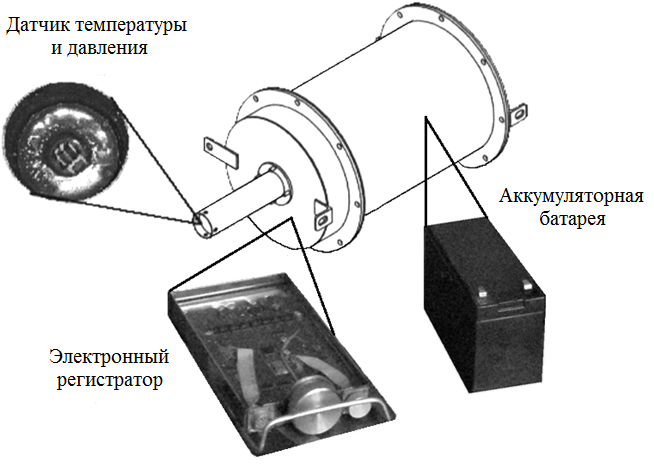
\includegraphics [scale=0.7] {ARV.png}
  \caption{Конструкция автономного регистратора придонного давления АРВ-К}
  \label{img:ARV}
\end{figure}


Данный прибор применяется для проведения натурных наблюдений волнения уже в течение 6 лет и зарекомендовал себя как надежный инструмент. Прибор обладает большим сроком автономной работы (6 мес.), относительно высокой частотой дискретизации (1 Гц ) и небольшой относительной погрешностью давления (0.06\%).

Более подробно принципы действия подобного средства измерения изложены в приложении \ref{AppendixA}, а также \cite{kovalev1993}.
%%%%END антиплагиат


\subsubsection{Способ постановки}

Автономный измеритель волнения, с помощью которого получены данные используемые в диссертации, ввиду принципа его работы размещается исходя из способов постановки притопленных измерителей волнения.

Сам измеритель располагается на дне, от него идет плавучий трос соединяющий его с якорем, который в свою очередь соединен с поверхностным буем. Такая схема постановки автономного измерителя волнения, приведена на рис. \ref{img:setSensor_1}.
\begin{figure} [h]
  \center
  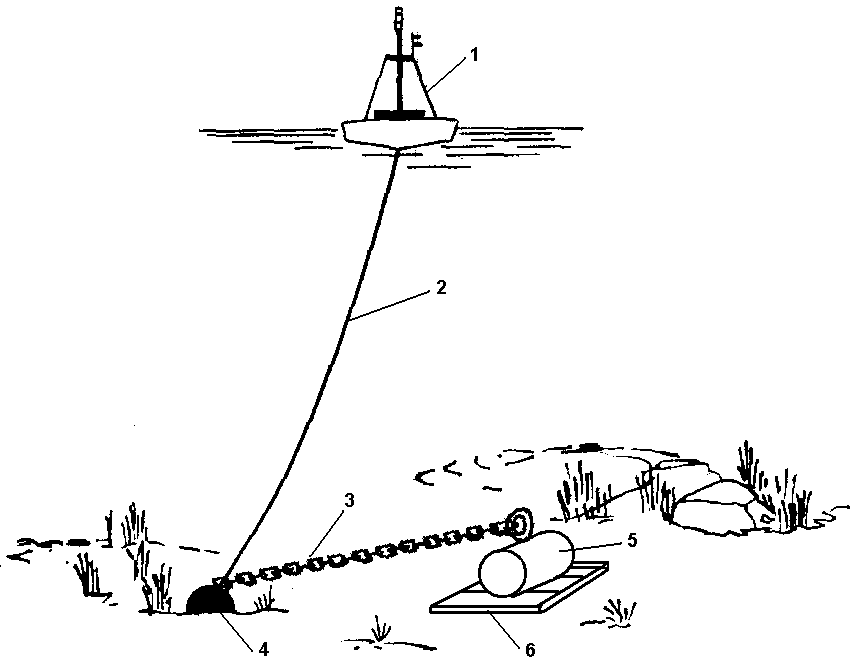
\includegraphics [width=0.5\linewidth] {setSensor_1.png}
  \caption{Схема постановки автономного регистратора волнения с использованием поверхностной буйковой станции. 1 -- поверхностный буй, 2 -- буйреп, 3 –- цепь, 4 -- якорь, 5 –- АРВ, 6 -– рама.}
  \label{img:setSensor_1}
\end{figure}
\FloatBarrier

Также измеритель волнения крепится на некоторый якорь или квадратную раму, который будет удерживать прибор от биений под действием придонных течений. На рис. \ref{img:setSensor_2} приведен внешний вид закрепленного на якоре автономного регистратора волнения для схемы постановки с использованием поверхностной буйковой станции, которые использовались при проведении мониторинга колебаний поверхности моря на Шельфе о.Сахалин.

\begin{figure} [h]
  \center
  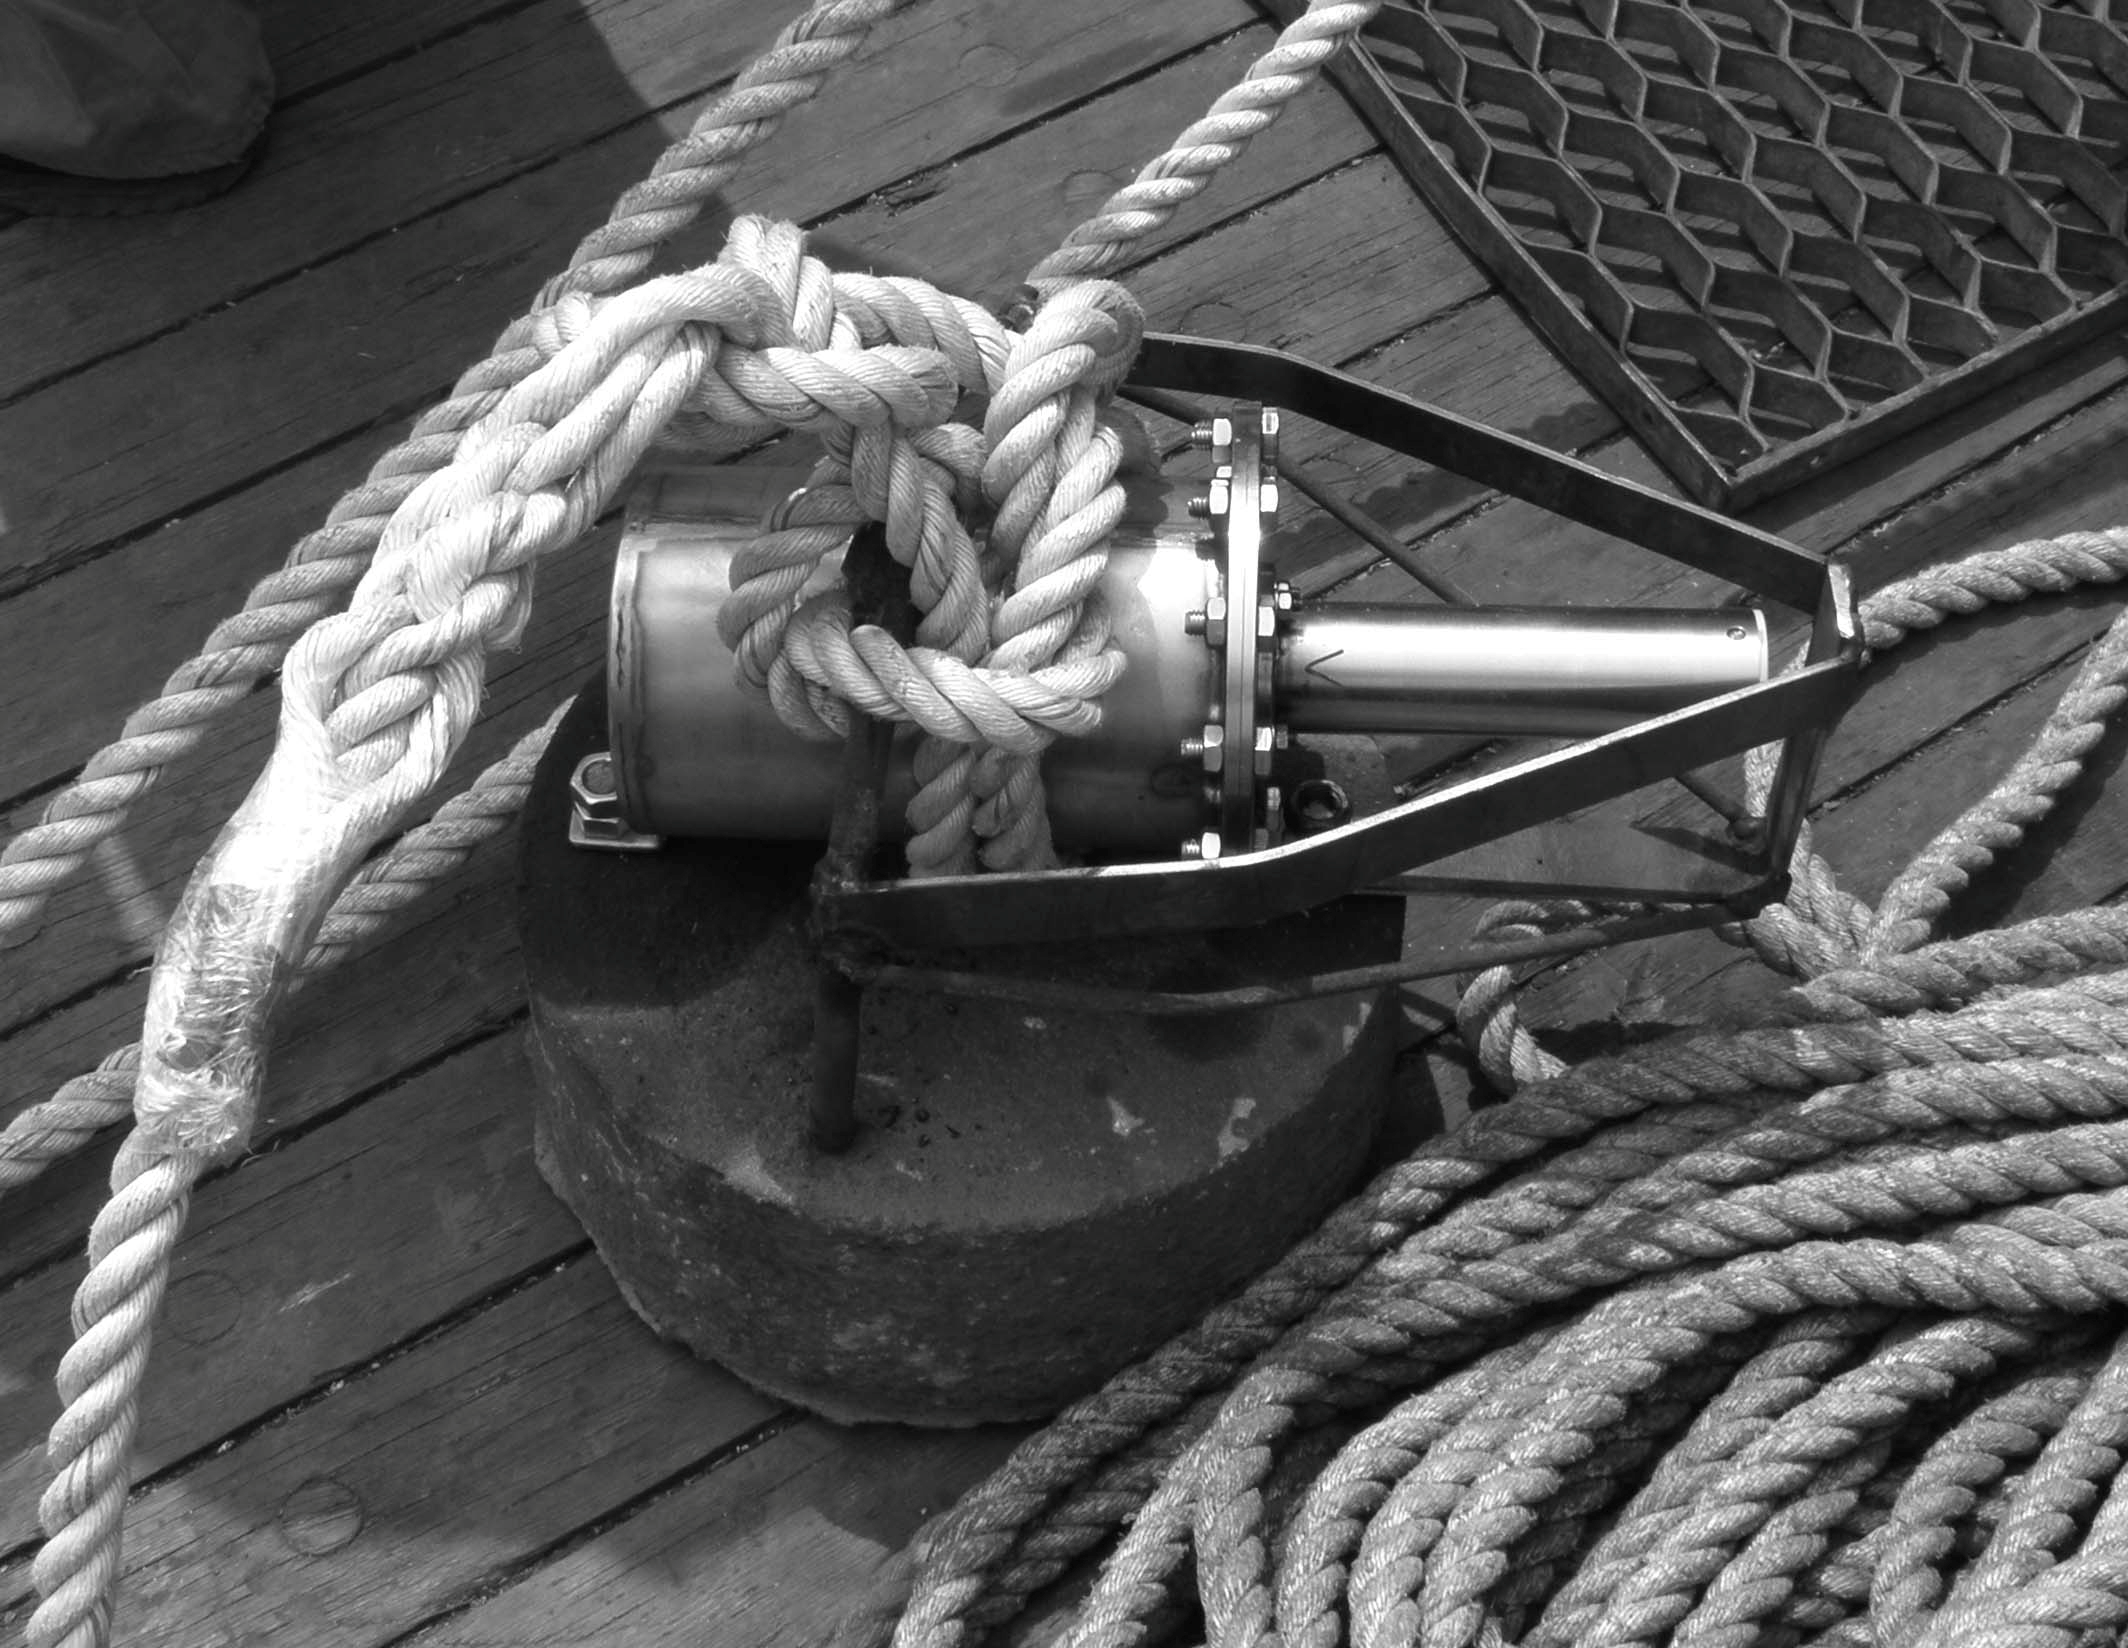
\includegraphics [width=0.5\linewidth] {setSensor_2.png}
  \caption{Внешний вид закрепленного на якоре прибора АРВ-К12.}
  \label{img:setSensor_2}
\end{figure}
\FloatBarrier

Иногда используют схему постановки в которой отсутствует дополнительный якорь, в таких случаях буй соединяется напрямую с измерителем.

При постановке также фиксируются координаты измерителя с помощью GPS-приемника. При подъеме поверхностный буй помогает определить точное местоположение прибора, так как иногда координат GPS-приемника недостаточно. После обнаружения измерителя, прибор вместе с якорем вытягивают со дна с помощью троса, идущего от буя.

В случае проведения измерений подо льдом, поверхностный буй размещают таким образом, чтобы он находился в толще воды, за несколько метров до поверхности, чтобы исключить прямое воздействие морского льда на буй. В таких случаях подъем поиск прибора существенно усложняется и может потребовать применения аквалангистов. Также, в таких случаях, эффективен метод траления с целью зацепить трос, идущий от прибора к якорю, с помощью крюков или кошки.

Главное преимущество притопленных измерителей заключается в том, что они обеспечивают более низкий уровень помех для измерений и лучшее качество получаемой информации, так как они не подвержены непосредственному воздействию ветра и поверхностных волн. По этой же причине притопленные измерители волнения обладают более высокой, чем поверхностные станции, надежностью.

Подробнее основные преимущества и недостатки обсуждаются в приложеннии к диссертации в разделе \ref{AppendexA_post}.


\subsection{Система регистрации волнения в режиме реального времени}

%%%%%Возможно подсократить и уба
Использование автономного прибора АРВ-К является удобным, так как установка и обслуживание являются достаточно нетрудоемкими. Установка прибора на дне моря продолжительностью 6 месяцев исключает передачу данных в режиме реального времени. СКБ САМИ ДВО РАН с 2010 года ведёт работы по передаче данных в режиме реального времени на сервер СКБ САМИ с последующей автоматической обработкой. В качестве полигона используется мыс Свободный. К настоящему времени выполнены работы по установке веб-камеры, которая в режиме реального времени также передаёт данные на сервер \url{www.skbsami.ru}. В 2011 году были проведены испытания прибора, позволяющего организовать регистрацию измерений и передачу данных \cite{Zaits_Kuz_NGTU_2013}. При организации наблюдений морского волнения в режиме реального времени на м. Свободный три основные проблемы:

\begin{enumerate}
  \item непостоянный источник электроэнергии, с высокой вероятностью перебоев в течение нескольких часов;
  \item нестабильная связь с местом натурных наблюдений, вызванная нестабильным и слабым сигнал сотовой станции;
  \item надежное подключение датчиков к береговому комплексу.
\end{enumerate}
Предложенная разработка позволяет решить эти проблемы, с помощью относительно недорогих  и, как показала практика, эффективных методов. На рис. \ref{img:autonomScheme} представлена принципиальная схема программно-аппаратного комплекса регистрации волнения в режиме реального времени.
\begin{figure} [h]
  \center
  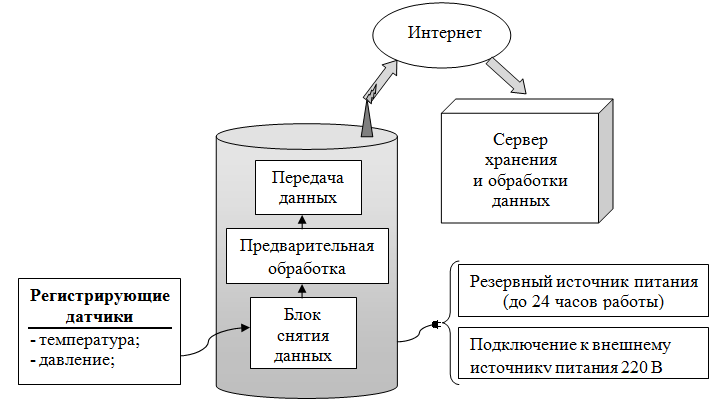
\includegraphics [scale=0.7] {autonomScheme.png}
  \caption{Принципиальная схема программно-аппаратного комплекса регистрации волнения в режиме реального времени}
  \label{img:autonomScheme}
\end{figure}
\FloatBarrier

В основе комплекса удаленного мониторинга морского волнения лежит персональный компьютер, выполненный в форм-факторе нетбука, с низкой потребляемой мощностью и достаточно большим временем автономной работы (15 часов). К нему подключается дополнительная аккумуляторная батарея, позволяющая существенно продлить срок автономной работы комплекса. К персональному компьютеру также подключен блок снятия данные обеспечивающий взаимодействие с регистрирующими датчиками, и блок передачи данных, который обеспечивает связь с сервером хранения и обработки данных. При этом на персональном компьютере осуществляется преобразование отсчетов подключенных датчиков в физические величины, а также сжатие данных в пакеты удобные для передачи на сервер. Подробнее про сервер хранения и обработки данных будет рассказано в разделе \ref{informSystem}.

Разработанная архитектура позволяет проводить регистрацию волнения, температуры и других параметров моря в режиме реального времени, в условиях крайне нестабильного энергопитания и плохого покрытия сотовой связью. В дальнейшем предполагается развертывание и поддерживание непрерывной работы разработанной системы. Технические подробности, разработанной системы описаны в \ref{AppendixA_Online}.


\section{Методы обработки результатов экспериментов}


При обработке результатов экспериментальных наблюдений и численного моделирования в настоящей работе использовался спектральный анализ, а также статистический анализ. Рассмотрим подробнее наиболее используемые в диссертации инструменты статистического и спектрального анализа.

\subsection{Проверка статистических гипотез}

Статистическая гипотеза представляет собой некоторое предположение о законе распределения случайной величины или о параметрах этого закона, формулируемое на основе выборки \cite{gmurman, leman, hodasev}. Гипотезы, в основе которых лежит допущение о конкретном виде закона распределения, называют параметрическими, в противном случае – непараметрическими. Гипотезу, утверждающую, что различие между сравниваемыми характеристиками отсутствует, а наблюдаемые отклонения объясняются лишь случайными колебаниями в выборках, на основании которых производится сравнение, называют нулевой (основной) гипотезой и обозначают $H_0$.

При этом если требуется проверить, согласуется ли множество выборочных значений с заданной гипотезой $H_0$, то мы рассматриваем распределение выборки и вычисляем некоторую подходящую меру $D\ge0$ отклонения этого распределения от гипотетического распределения. По выборочному распределению величины $D$ мы определяем критическое значение $D_0$, такое, что если гипотеза $H_0$  верна, то $P(D>D_0)=\alpha$, где $\alpha$ -- заранее заданный уровень значимости. Если в конкретном случае мы обнаружим отклонение $D>D_0$, то гипотеза $H_0$ отвергается, в то время как появление значения $D\le D_0$ считается совместимым с гипотезой $H_0$, которая тогда принимается.

Приняв это правило, мы с вероятностью, равной $\alpha$, можем отвергнуть в действительности справедливую гипотезу $H_0$, поскольку $\alpha$ можно выбрать сколь угодно малой. Для избежания таких ситуаций необходимо очень внимательно относиться к выбираемому уровню значимости $\alpha$ и мере отклонения $D$ или подходящему критерию.

В зависимости от сущности проверяемой гипотезы и используемых мер расхождения оценки характеристики от ее теоретического значения применяют различные критерии. К числу наиболее часто применяемых критериев для проверки гипотез о законах распределения относят критерии $\chi^2$ Пирсона, Колмогорова, Мизеса, Вилкоксона, о значениях параметров – критерии Фишера, Стьюдента.

При объеме выборки $n>40$ для проверки гипотезы о законе распределения используют критерий $\chi^2$ (критерий Пирсона, критерий согласия). Он применяется для группированных данных (как при построении гистограммы), когда в каждом интервале находится не менее 5 измерений (иначе интервал называется малонаселенным). Если число измерений в интервале оказывается меньше 5, тогда он объединяется с соседним.

%Современный взгляд на этот вопрос заключается в следующем: не должно быть «пустых» интервалов [8].

Если рассматривать частоту $i$-го интервала как случайную величину, то  $n_i$ –- число появлений «успеха» в  независимых испытаниях, где под «успехом» понимается попадание случайной величины $X$ в $i$-й интервал. Таким образом, вероятность «успеха» равна $P_i$, а случайная величина $X$ имеет биномиальное распределение с параметрами $n$ и $P_i$.

Рассмотрим статистику $\chi^2$ –- функцию от случайных величин $n_1, n_2,n_3,...,n_k$, определяемую формулой
\begin{equation}\label{eq:chi}
  \chi^2=\sum\limits_{i=1}^k\frac{(n_i-nP_i)^2}{nP_i},
\end{equation}
где $n_i$ -- число данных в $i$-м интервале $(i=1,n)$, $P_i$ -- теоретическая вероятность попадания случайной величины $X$ в $i$-й интервал, $n$ -- объем выборки, $k$ -- число интервалов.

Можно показать, что, если закон распределения генеральной совокупности $X$ подобран правильно, то с ростом $n$ случайную величину $X$ можно считать распределенной по распределению $\chi_{\nu}^2$ с числом степеней свободы $\nu=k-r-1$; $r$ -– числом параметров проверяемого закона распределения, вычисленных по выборке. Следует обратить внимание на то, что число степеней свободы -- это число независимых слагаемых в сумме \eqref{eq:chi}, т.е. общее число слагаемых минус число наложенных уравнений уравнений связи. В общем случае по выборке оценивают $r$ параметров.

Еще одно уравнение связи вполне очевидно: сумма всех вероятностей $P_i$ равна 1 или некоторому числу меньшему 1 (но известному). Так в случае наиболее часто рассматриваемого в диссертации распределения Вэйбулла \eqref{eq:weib} $r=2$, так как по выборке оцениваются два параметра распределения.
\begin{equation} \label{eq:weib}
F(X)=1-\exp \left[-b\left(X \right)^{p} \right]
\end{equation}

Итак критерий согласия $\chi^2$ имеет вид
\begin{equation}\label{eq:chiCrit}
  \chi^2=\sum\limits_{i=1}^k\frac{(n_i-nP_i)^2}{nP_i}\le\chi_{\nu,кр}^2,
\end{equation}

Вычисленное по формуле \eqref{eq:chiCrit} значение сравнивается с табличным (критическим) при выбранном одностороннем уровне значимости $\alpha$. Если $\chi^2\le\chi_{\nu,кр}^2$, то гипотеза $H_0$ в виде распределения не отвергается, в противном случае она отвергается, и строится новая гипотеза -- предполагается другой закон распределения.

При этом стоит отметить что статистика $\chi^2$ лишь приближенно имеет распределение $\chi^2_{\nu}$ (при справедливой нулевой гипотезе), причем для этого необходим не только большой объем выборки $n$, но и достаточно большое число интервалов $r$. В случае когда эти значения $n$ и $r$ недостаточно большие критерий \eqref{eq:chiCrit} обладает повышенной вероятностью ошибки первого рода  (признать неверной проверяемую нулевую гипотезу, когда она верна).

\subsection{ Спектральный анализ записей}

Спектральный анализ волнограмм морского волнения позволяет  в частотной области исследовать особенности развития различных процессов. Рассмотрим подробнее методы спектрального анализа, основанные на преобразовании Фурье.

Преобразование Фурье удобно представлять в следующей форме:
\begin{equation}\label{eq:fourier}
  S(\omega)=\int\limits^{+\infty}_{-\infty}\eta(t)\exp(-i\omega t)dt,
\end{equation}
\noindent
где $\omega$ -- круговая частота, $\eta(t)$ -- колебания поверхности жидкости от времени.  При этом величину $S(\omega)$ называют спектральной функцией, а ее модуль $|S(\omega)|$ -- \emph{амплитудным спектром}.

При обработке экспериментальных данных приходится иметь дело не с аналитическими функциями, а с дискретными данными, в этом случае необходимо использовать дискретное преобразование Фурье:

\begin{equation}\label{eq:fourierDiscr}
  S_k=\sum\limits^{N-1}_{n=0}\eta_n\exp(-i\frac{2\pi}{N}kn),
  k=0,1,..,N-1,
\end{equation}
\noindent
где $\eta_n$ -- измеренные значения смещения поверхности, в дискретных временных точках с номерами $n=0,1,...,N-1$;
$N$ -- количество значений анализируемого сигнала, полученного за нужный период измерений;
$k$ -- индекс частоты, частота $k$-ой гармоники равна $k/T$, где $T$ -- временной интервал наблюдения анализируемого сигнала;
$S_k$ -- комплексные амплитуды синусоидальных сигналов, слагающих исходный сигнал ($k=0,1,...,N-1$).

При этом отношение $S_k/N$ -- будет являться обычной вещественной амплитудой $k$-ой гармоники исходного сигнала, а $\arg(S_k)$ -- фаза $k$-ой гармоники исходного сигнала.

При спектральном анализе случайных сигналов основной целью является определение \emph{спектральной плотности мощности} (СПМ).

Прямой метод определения СПМ случайных последовательностей основан на вычислении квадрата модуля дискретного преобразования Фурье отдельных участков последовательности данных с использованием соответствующего статистического усреднения (метод периодограмм).

Выборочная спектральная плотность мощности случайного процесса $\eta(t)$, с реализацией последовательностью конечной длины $\eta_0,\eta_1,...,\eta_{N-1}$, описывается выражением:

\begin{equation}\label{eq:psd}
  \hat{G}_k = \frac{|S_k|^2}{N\Delta t},
\end{equation}
\noindent
где $S_k$ -- дискретное во времени преобразование Фурье, определяемое формулой \eqref{eq:fourierDiscr}; $\Delta t$ -- частота дискретизации, которую можно описать как $T/N$.

Можно оценить размерность этой величины $\hat{G}_k$ в предположении, что уровень оцениваемого сигнала имеет размерность [метр], а продолжительность наблюдений - [секунда]. В этом случае размерность величины $S_k$ дискретного преобразование Фурье \eqref{eq:fourierDiscr} является $[\text{м}\times\text{с}]$, тогда размерность величины $\hat{G}_k$, можно выразить как:
$$
[\hat{G}_k]=\left[\frac{\text{м}^2\times\text{с}^2}{\text{с}}\right]=[\text{м}^2\times\text{с}].
$$


\subsubsection{Метод Уэлча }


%%%%ПЕреработать нужный блок!
Для уменьшения этой изрезанности необходимо применить какое--либо усреднение.
Итак, вычисления при использовании метода Уэлча (он называется еще методом усреднения модифицированных периодограмм -- averaged modified periodogram method) организуются следующим образом:

\begin{enumerate}
\item  Запись делится на перекрывающиеся сегменты. Как правило, на практике используется перекрытие на 50 \%. Строго говоря, оптимальная степень перекрытия зависит от используемой весовой функции.

\item  Каждый сегмент умножается на используемую весовую функцию.

\item  Для взвешенных сегментов вычисляются модифицированные периодограммы.

\item  Периодограммы всех сегментов усредняются.
\end{enumerate}

Дисперсия оценки, получаемой методом Уэлча, уменьшается примерно пропорционально числу сегментов. Благодаря перекрытию в методе Уэлча используется больше сегментов, поэтому снижается дисперсия оценки спектра плотности мощности.


\subsubsection{Текущий спектр}

Проводя спектральный анализ записи с помощью методов описанных выше, мы получаем усредненные оценки этой записи. Реальное морское волнение сильно изменчиво во времени, со временем изменяются в том числе и спектральные характеристики. Иногда наиболее интересными, при изучении спектральных характеристик морского волнения, являются моменты изменения спектральных характеристик. Таким образом наиболее необходим инструмент спектрального анализа, который позволяет отследить временную изменчивость спектральных характеристик записи и развитие периодических процессов во времени.

Такую спектрально-временную диаграмму, выражающую зависимость спектральной характеристики от времени называют \emph{текущим спектром}, его можно описать через следующее преобразование:

\begin{equation}\label{eq:currSpectr}
  S(\omega,t)=\int\limits^{t}_0\eta(t)\exp(-i\omega t)dt,
\end{equation}

На практике, когда необходимо произвести спектрально-временную оценку дискретного сигнала обычно применяют методы, основанные на спектральном оценивании с помощью периодограмм Уэлча, описанных выше.

Опишем алгоритм, который позволяет получить спектрально-временную оценку записи.
\begin{enumerate}
  \item Ряд данных разбивается на перекрывающиеся сегменты, наиболее оптимальным оказывается использование перекрытия на 40\%.
  \item Для каждого выделенного сегмента производится спектральная оценка по методу периодограммы Уэлча. Такой подход позволяет получить максимально точную оценку спектральную оценку в конечном результате.
  \item Вычисленные значение спектральных составляющих заносятся в двумерный массив, который имеет размер $N\times M$, где $N$ -- количество частот, $M$ -- количество сегментов, которое будет отражать временную зависимость.
  \item Двумерный массив отображается как поверхность, где по оси $X$ идет время, по оси $Y$ – период, а по $Z$ – спектр, с логарифмической шкалой по этой оси.
\end{enumerate}
Пример расчитанных по этому алгоритму текущие спектров можно увидеть в Главе 2 (Рис.\ref{img:svobodny_3}, Рис.\ref{img:svobodny_4}, Рис.\ref{img:vzmorie_2}, Рис.\ref{img:vzmorie_3} и т.д.), где они подробно анализируются.



\section{Информационная система хранения и обработки данных}\label{informSystem}

Основным инструментом измерений стал автономный регистратор волнения \textcolor[rgb]{1.00,0.00,0.00}{[6]}, основанный на измерении пульсации давления под водой, индуцированной поверхностными волнами. За несколько лет эксплуатации прибор зарекомендовал себя как инструмент, обладающий высокой надежностью, простотой обращения, качеством получаемых данных и относительной дешевизной. Результатом работы прибора на протяжении пяти с половиной месяцев является текстовый файл, содержащий время, придонное давление и температуру с дискретностью одна секунда, размер одного файла составляет около 700 мегабайт. За годы проводимых натурных наблюдений скопился очень большой объём данных (порядка 170 гигабайт), с которыми довольно затруднительно работать, поскольку приходится использовать различные программы и приложения для обработки результатов. Эти программы громоздки и медлительны, что в итоге служит серьезным сдерживающим фактором при анализе данных. Все вышеизложенное свидетельствует о необходимости разработки информационной системы, позволяющей, в первую очередь структурировано хранить данные и предоставлять к ним удобный доступ, а также проводить типовую обработку океанологических данных.

В настоящее время наиболее известными российскими базами океанографических данных являются база ТОИ ДВО РАН «ОКЕАН-1» и «ОКЕАН-2»  и база Института океанологии им. П.П. Ширшова РАН \textcolor[rgb]{1.00,0.00,0.00}{(ссылки на базу)}. Однако эти базы ориентированы на другие задачи и не позволяют выполнять требуемые операции, такие как получение необходимого временного ряда за заданный промежуток времени и проведение типовой обработки.

Таким образом, для решения, описанных выше задач была разработана информационная система хранения и обработки данных, полученных в результате натурных измерений волнения, названная OceanData. С точки зрения информационных технологий OceanData представляет собой сложный расчетный программный комплекс с модульной архитектурой. В качестве основных единиц декомпозиции продукта можно выделить следующие:
\begin{itemize}
  \item блок хранения данных;
  \item пользовательский интерфейс представленный в виде сайта;
  \item блок обработки данных (набор оптимизированных программ);
  \item блок управления запросами пользователя (набор php-скриптов).
\end{itemize}

\subsubsection{Архитектура системы}

В основе архитектуры системы лежит клиент-серверная технология. Соответственно, выделяют клиентскую и серверную стороны приложения. Клиентская сторона приложения функционирует на рабочем месте пользователя, в роли которого выступает браузер персонального компьютера. Серверная сторона функционирует на специализированном комплексе, включающем в себя мощные аппаратные средства, требуемый набор стандартного программного обеспечения, систему управления базами данных и собственно структуры данных. На рис. \ref{img:arch} изображено послойное представление архитектуры системы.
\begin{figure} [h]
  \center
  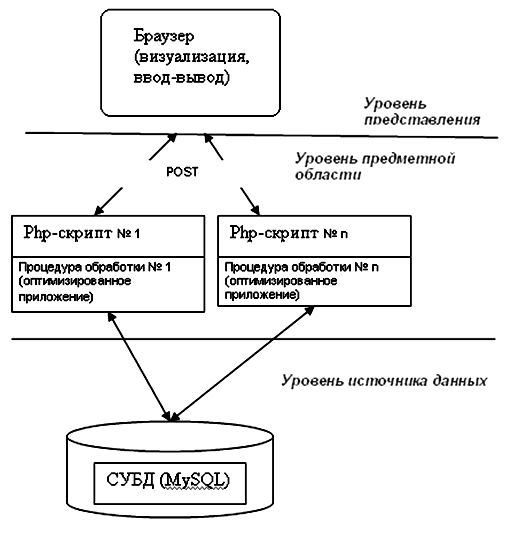
\includegraphics [scale=0.7] {architecture.png}
  \caption{Послойное представление архитектуры системы}
  \label{img:arch}
\end{figure}
\FloatBarrier
Взаимодействие клиентской и серверной частей приложения осуществляется через сеть – локальную или глобальную. При этом с точки зрения клиента и сервера взаимодействие осуществляется прозрачно, соответственно сетевой компонент включает в себя совокупность необходимого сетевого оборудования, набор программных технологий, обеспечивающих передачу данных между узлами сети, а также собственно протокол или протоколы для обмена запросами и результатами их выполнения.

Система состоит из трех слоев или компонент:
\begin{itemize}
  \item компонент ввода-вывода,
  \item компонент прикладной логики,
  \item компонент хранения базы данных
\end{itemize}

При этом компонент прикладной логики находится на промежуточном слое, который является клиентом для базы данных и сервером для пользователя. На стороне пользователя выполняются только операции визуализации и ввода-вывода данных, а всю прикладную логику реализует сервер. Обмен между клиентом и сервером в таких системах осуществляется на уровне команд вывода данных на экран и результатов пользовательского ввода.

Пользователь, набрав в браузере адрес системы http://hydrolab.nnov.ru/, получает доступ к пользовательскому интерфейсу системы. Удобный интерфейс позволяет ему сформировать нужные запросы к базе, не требуя при этом специальных знаний. Запрос отправляется на сервер системы, где его обрабатывает php-скрипт. Скрипт проводит интерпретацию и проверку полученных данных, после чего запускает оптимизированное приложение с нужными параметрами. Приложение, общаясь напрямую с базой данных, записывает или читает данные из базы и проводит над ними процедуру обработки.

Далее представлены некоторые особенности реализации отдельных модулей программного обеспечения.

\subsubsection{Особенности реализации}

%%%%Возможно подробнее про это!
Хранение и управление данными осуществляет СУБД MySQL. Основная таблица базы данных – таблица паспорта эксперимента, в которой хранится полная информация о месте и времени проведения эксперимента, а также об элементах датчика, с которого получена запись. С каждой записью в этой таблице ассоциирована другая таблица, содержащая следующие атрибуты: давление, температуру и время записи.

\emph{Картинка структуры базы данных}


Поскольку основной задачей системы является структурированное хранение данных об экспериментах и удобный доступ к ним, основными функциями являются импорт и экспорт из базы данных. Остановимся подробнее их реализацию. При импорте данных скорость не так важна, поскольку эта операция используется сравнительно редко. При экспорте скорость обработки играет, куда большую роль. По запросу пользователя программа обращается к базе данных, запрашивая нужный временной ряд. Полученный ряд, сглаживается заданным пользователем окном с помощью алгоритма Кайзера-Бесселя, потом записывается в текстовый файл, который сжимается архиватором, затем пользователю выдается ссылка на скачивание файла. Поскольку объем данных, которыми приходится часто оперировать достаточно большой (средний размер запрашиваемого файла с данными около 60 мегабайт), необходимо максимально оптимизировать работу с ними. Выборка нужного временного интервала происходит с помощью программы, реализованной на C++. При этом дополнительно используются оптимизированные библиотеки Intel Performance Primitives, позволяющие сократить скорость время выполнения некоторых алгоритмов в десять раз по сравнению с неоптимизированной их реализацией.
%%%%Возможно подробнее про Intel...

Также существенно снижается, время выполнения операции экспорта из базы данных при записи файла не на жесткий диск, а в оперативную память, так как скорость записи в ПЗУ в десятки раз быстрее. Для того чтобы максимально использовать эту особенность можно задействовать специальную файловая система tmpfs. Данная файловая система монтируется на нужную папку, ассоциируя при этом все файлы внутри этой папки с областью оперативной памяти. Позволяя таким образом все операции чтения-записи в эту папку вести со скоростью оперативной памяти. Tmpfs позволяет резервировать в оперативной памяти место, определенного объема, после переполнения которого файлы автоматически начинают записываться на жесткий диск.

Общение между сервером и клиентами происходит через php-скрипты. С каждой операцией и методикой ассоциирован свой php-скрипт, проводящий проверку введенных пользователем данных и запускающий оптимизированную процедуру обработки. Подобный подход позволяет легко расширять систему, поскольку для добавления новой методики не требуется изменения уже существующих скриптов и программного кода.

Следующая задача – обзор и анализ данных. Для нее реализована возможность графического представления данных об экспериментах. Это в первую очередь отображение мест постановок датчиков на карте, а также построение графиков давления и придонной температуры. Для отображения данных на карте используется продукт компании Google – Google-Maps, а также средства для разработчиков, позволяющие использовать в своих приложениях этот продукт – API Maps. Отображение на карте позволяет оценить расстояние между датчиками, а также дает возможность оценить пространственную структуру процессов, зарегистрированных датчиками.
Для построения графиков давления и температуры использована программа gnuplot, считывающая данные из файла, находящегося под управлением файловой системы tmpfs, описанной выше. Gnuplot несколько лет занимает лидирующие позиции среди программ построения графиков и используется огромным количеством организаций. В результате работы программы пользователю предоставляются качественные графики, практически готовые к публикации. При построении графиков используются только те данные, которые возможно отобразить на изображении заданного разрешения, в результате время выполнения снижается в несколько раз без потери качества графика.

Пользовательский интерфейс представляет собой сайт, находящий под управлением «Joomla! CMS». Выбор именно этой системы управления сайтами обусловлен тем, что на сегодняшний день эта CMS является наиболее гибкой и надежной. Ее распространение повлекло за собой появление огромного количества дополнений и плагинов для этой системы, которые позволяют легко добавлять новые функциональные возможности на сайт.

Интерфейс реализован с применением технологии AJAX (Asynchronous Javascript and XML), позволяющей производить запросы на сервер без перезагрузки всей страницы. На рис. \ref{img:interface} представлен процесс построения графика нужного временного ряда.
\begin{figure} [h]
  \center
  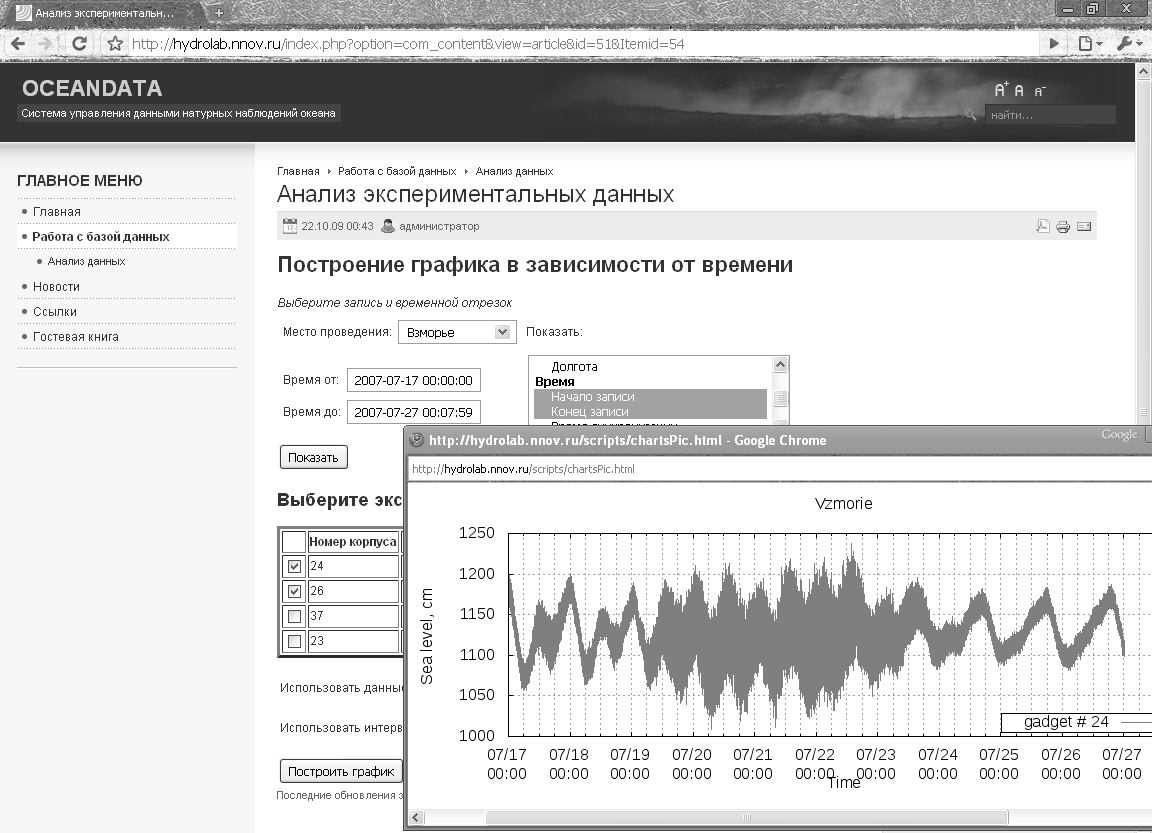
\includegraphics [width=170 mm] {interface.png}
  \caption{Послойное представление архитектуры системы}
  \label{img:interface}
\end{figure}
\FloatBarrier
Интерфейс предоставляет возможность авторизации пользователей и предоставление им доступа к различным функциям системы. Незарегистрированные пользователи смогут посмотреть расположение датчиков на карте и построить график нужного временного ряда. Функция экспорта из базы данных и добавления новых экспериментов доступны только авторизованным пользователям.


\section{Заключение}

%%%Заключение по всей главе:
%%1. Показаны уравнения
%%2. Представлены и т.д.
%%%Блок заключения по инф. системе:
Подобная система позволяет структурировать и упорядочить собранные океанологические данные. Удобный доступ с помощью пользовательского интерфейса существенно упрощает работу с ними. Дополнительный плюс системы в том, что доступ к данным возможен с любого компьютера и из любой точки мира, при этом не требуется дополнительного программного обеспечения. Система позволяет пользователю получить данные с любой дискретностью в виде тестового файла с выбранными рядами данных. С такими файлами работает любая программа обработки данных. Подобный подход предоставляет пользователю абсолютную свободу в выборе программного инструмента для дальнейшей работы. Представление мест постановок на карте позволяет проводить пространственный анализ волновых процессов. Большое внимание при разработке системы было уделено скорости обработки, а для максимальной эффективности, применялись последние разработки компании Intel в этой области.
В настоящий момент описанная информационная система прошла тестирование и полностью функционирует, и активно используется сотрудниками НГТУ им.Р.Е.Алексеева и ИМГиГ ДВО РАН при проведении натурных экспериментов на шельфе дальневосточных морей России. Дальнейшая работа будет связана с наполнением базы результатами новых экспериментов, добавлением возможности хранения метеоданных и наращиванием функционала системы.

\clearpage
